\documentclass[10pt,conference,compsoc]{IEEEtran}

\usepackage{amsmath,amssymb,amsfonts}
\usepackage{algorithmic}
\usepackage{algorithm}
\usepackage{graphicx}
\usepackage{textcomp}
\usepackage{xcolor}
\usepackage{booktabs}
\usepackage{multirow}
\usepackage{multicol}
\usepackage{microtype}
\usepackage{url}
\usepackage{hyperref}

\hypersetup{hidelinks}

\begin{document}

\title{Comparative Empirical Evaluation of Ensemble Learning Architectures for Network Intrusion Detection on UNSW-NB15 Telemetry}

\author{\IEEEauthorblockN{Student Number: 24888923}
\IEEEauthorblockA{\textit{Department of Mathematical Sciences (Computer Science Division)} \\
\textit{Stellenbosch University}, Stellenbosch, South Africa \\
Email: 24888923@sun.ac.za}
}

\maketitle

\begin{abstract}
High-throughput network intrusion detection systems require robust classification accuracy across diverse and heavily imbalanced cyberattack categories. This study evaluates three ensemble learning architectures, namely random forests (RF), gradient boosted decision trees (GBDT), and heterogeneous stacking ensembles, against baseline single classification and regression trees (CART) and k-nearest neighbours (kNN) models on 257,673 instances of UNSW-NB15 network telemetry. The empirical evaluation protocol incorporates five-fold stratified cross-validation, cost-sensitive Gini impurity class weighting, and non-parametric statistical hypothesis testing comprising the Friedman omnibus test and Nemenyi \textit{post hoc} critical difference analysis. Experimental findings demonstrate that random forest ensembling achieves superior generalization performance, attaining a macro $\text{F}_1$-score of 0.6842 $\pm$ 0.0085. This represents a statistically significant improvement of +10.81 percentage points over single decision trees and +23.65 percentage points over k-nearest neighbours. Additionally, random forest ensembling elevates minority Worms attack recall from 0.5575 to 0.8241 while maintaining real-time packet processing throughput. Algorithmic code implementations and experimental replication scripts are accessible in the project repository.\footnote{\url{https://github.com/TomDesHeath/machine-learning-441-assignment4}}
\end{abstract}

\section{Introduction}

Automated intrusion detection systems operating on high-rate computer network telemetry require reliable identification of complex cyberattack signatures. Single-estimator machine learning models frequently exhibit structural limitations when trained on high-dimensional network telemetry. Classification and regression trees (CART) suffer from high estimation variance and structural instability, wherein minor perturbations in training traffic yield disparate partition structures. Conversely, k-nearest neighbours (kNN) algorithms incur severe computational latency during query inference and suffer degraded distance metrics across high-dimensional feature spaces.

Ensemble learning architectures mitigate single-estimator limitations by combining predictions from multiple base learners. Homogeneous bagging ensembles, such as random forests (RF), reduce variance through bootstrap aggregation and feature subspace sampling. Homogeneous boosting ensembles, such as multi-class gradient boosted decision trees (GBDT), iteratively reduce bias by fitting successive regression trees to negative loss gradients. Heterogeneous stacking ensembles blend probability outputs from distinct algorithmic families using a meta-learner.

This investigation conducts an empirical comparison of random forests, gradient boosted decision trees, and stacking meta-learners against single decision tree and k-nearest neighbour baselines on the UNSW-NB15 dataset. The investigation focuses on three primary scientific inquiries. First, whether random forest ensembling systematically reduces generalization variance and eliminates minority-class overfitting compared to single decision trees on network telemetry. Second, how sequential error targeting in gradient boosting compares to parallel variance reduction in random forests under severe target class imbalance. Third, the quantitative trade-off between ensemble inference throughput and multi-class classification accuracy in real-time network monitoring.

The remainder of this report is organized as follows. Section II details theoretical background, dataset characteristics, mathematical ensemble formulations, and non-parametric statistical testing protocols. Section III presents computational design, vectorization strategies, and formal algorithmic implementations. Section IV outlines empirical methodology and hyperparameter tuning configurations. Section V presents experimental results, statistical hypothesis evaluations, and detailed analyses of the core scientific inquiries. Section VI concludes with operational deployment recommendations. Appendix A provides acronym definitions, and Appendix B details mathematical notation.

\section{Theoretical Background}

This section provides the theoretical foundation for the study, detailing telemetry dataset characteristics, mathematical formulations of single and ensemble classifiers, and the non-parametric statistical framework. The discussion begins with telemetry data quality challenges, proceeds to classifier formulations, and concludes with statistical hypothesis testing protocols.

\subsection{Dataset Quality Challenges in Network Telemetry}
The UNSW-NB15 telemetry dataset, introduced by Moustafa and Slay \cite{moustafa2015}, comprises $N = 257,673$ traffic flow observations spanning $D = 43$ descriptive features and $C = 10$ target categories ($C \in \{0, 1, \dots, 9\}$). Network telemetry exhibits five primary data quality challenges that influence model induction.

First, missing nominal attributes occur in the \texttt{service} feature, which contains 141,321 missing entries recorded as \texttt{?}. Imputation with mode values distorts domain semantics, and missingness is consequently encoded as an explicit categorical level \texttt{missing}. Second, collinear descriptors arise because byte volume metrics (\texttt{sbytes}, \texttt{dbytes}) and packet volume metrics (\texttt{spkts}, \texttt{dpkts}) exhibit strong linear dependence. Tree-based partitioning naturally mitigates collinearity by selecting individual features at split nodes. Third, uninformative identifiers such as the \texttt{id} attribute represent arbitrary database row indices and are excluded prior to model induction. Fourth, extreme positive skewness affects duration (\texttt{dur}) and transaction rate (\texttt{rate}), which span multiple orders of magnitude. Tree-based models maintain monotonic scale invariance, eliminating the necessity for non-linear power transformations. Fifth, extreme class imbalance characterizes the target distribution, which ranges from Normal background traffic (36.09\%, $N=93,000$) and Generic attacks (22.85\%, $N=58,871$) down to rare attack categories such as Shellcode (0.59\%, $N=1,511$) and Worms (0.07\%, $N=174$).

\subsection{Single-Estimator Classifier Formulations}
Classification trees recursively partition sample space $S$ into orthogonal axis-aligned hyper-rectangles, as formulated by Quinlan \cite{quinlan1986}. At node $m$ containing subset $Q_m$, optimal split feature $j^*$ and threshold $t^*$ maximize weighted Gini impurity reduction:
\begin{equation}
\Delta I(m, j, t) = W_m G(Q_m) - W_L G(Q_L) - W_R G(Q_R),
\end{equation}
where $W_m = \sum_{i \in Q_m} w_i$ represents sample weight sum. Gini impurity $G(Q_m)$ is computed as:
\begin{equation}
G(Q_m) = 1 - \sum_{c=0}^{C-1} p_{mc}^2, \quad p_{mc} = \frac{\sum_{i \in Q_m, y_i=c} w_i}{W_m}.
\end{equation}
To address class imbalance, balanced class weights are assigned as $w_c = \frac{N}{C \cdot N_c}$.

The k-nearest neighbours algorithm assigns class labels via Minkowski distance ($p=2$) over reference training set $D_{tr}$:
\begin{equation}
\hat{y}(\mathbf{x}) = \arg\max_{c \in \{0,\dots,C-1\}} \sum_{i \in \mathcal{N}_k(\mathbf{x})} \frac{1}{d(\mathbf{x}, \mathbf{x}_i) + \epsilon} I(y_i = c),
\end{equation}
where $\mathcal{N}_k(\mathbf{x})$ denotes the set of $k$ closest training vectors to query instance $\mathbf{x}$, and $\epsilon > 0$ prevents division by zero.

\subsection{Random Forest Ensembling}
Random forest ensembling constructs $M$ decision trees trained on bootstrap samples $D_m \sim D$, as formulated by Breiman \cite{breiman2001}. Diversity is introduced via dual randomization mechanisms. In bootstrap aggregation, each member tree $h_m(\mathbf{x})$ is induced on a bootstrap sample of size $N$ drawn with replacement from $D$. In random subspace selection, each candidate split node evaluates a random feature subset of size $m_{\text{feat}} = \lfloor \sqrt{D} \rfloor$.

Final class predictions combine tree probability outputs via majority voting:
\begin{equation}
H_{\text{RF}}(\mathbf{x}) = \arg\max_{c \in \{0,\dots,C-1\}} \frac{1}{M} \sum_{m=1}^M I(h_m(\mathbf{x}) = c).
\end{equation}
Out-of-bag generalization error $E_{\text{OOB}}$ evaluates model generalization without cross-validation by testing observation $\mathbf{x}_i$ exclusively on trees where $\mathbf{x}_i \notin D_m$, as shown by Breiman \cite{breiman2001}:
\begin{equation}
E_{\text{OOB}} = \frac{1}{N} \sum_{i=1}^N I\Bigl( \arg\max_{c} \sum_{m: \mathbf{x}_i \notin D_m} I(h_m(\mathbf{x}_i) = c) \neq y_i \Bigr).
\end{equation}

\subsection{Multi-Class Gradient Boosted Decision Trees}
Multi-class gradient boosted decision trees maintain $C$ additive continuous score functions $f_0(\mathbf{x}), \dots, f_{C-1}(\mathbf{x})$, following Friedman \cite{friedman2001}. Class probabilities follow the softmax transformation:
\begin{equation}
p_c(\mathbf{x}) = \frac{\exp(f_c(\mathbf{x}))}{\sum_{k=0}^{C-1} \exp(f_k(\mathbf{x}))}.
\end{equation}
The objective minimizes multinomial cross-entropy loss $L(y, \mathbf{f}(\mathbf{x})) = -\sum_{c=0}^{C-1} y_c \ln p_c(\mathbf{x})$. At iteration $m$, negative gradients representing pseudo-residuals are evaluated for observation $i$ and class $c$:
\begin{equation}
r_{ic}^{(m)} = -\left[ \frac{\partial L(y_i, \mathbf{f}(\mathbf{x}_i))}{\partial f_c(\mathbf{x}_i)} \right]_{\mathbf{f}=\mathbf{f}^{(m-1)}} = y_{ic} - p_c^{(m-1)}(\mathbf{x}_i).
\end{equation}
A regression tree $h_{mc}(\mathbf{x})$ is fit to pseudo-residuals $r_{ic}^{(m)}$. Terminal leaf values $\gamma_{jmc}$ are updated via Newton-Raphson line search:
\begin{equation}
\gamma_{jmc} = \frac{C-1}{C} \frac{\sum_{\mathbf{x}_i \in R_{jmc}} r_{ic}^{(m)}}{\sum_{\mathbf{x}_i \in R_{jmc}} p_{ic}^{(m-1)} (1 - p_{ic}^{(m-1)})}.
\end{equation}
Ensemble scores advance with shrinkage learning rate $\eta \in (0, 1]$:
\begin{equation}
f_c^{(m)}(\mathbf{x}) = f_c^{(m-1)}(\mathbf{x}) + \eta \cdot h_{mc}(\mathbf{x}).
\end{equation}

\subsection{Heterogeneous Stacking Ensembles}
Stacking ensembles organize estimation into a two-tier hierarchy, as formulated by Wolpert \cite{wolpert1992}. In Level-0, $K$ base models generate out-of-fold class probability matrices $\mathbf{Z}_{\text{OOF}} \in \mathbb{R}^{N \times (K \cdot C)}$ using five-fold cross-validation. In Level-1, a meta-classifier $g_{\text{meta}}$, implemented as multinomial logistic regression with $L_2$ regularization, fits on meta-features $\mathbf{Z}_{\text{OOF}}$ to yield final predictions:
\begin{equation}
\hat{y}_{\text{stack}}(\mathbf{x}) = g_{\text{meta}}\left( [\hat{\mathbf{p}}_1(\mathbf{x}), \dots, \hat{\mathbf{p}}_K(\mathbf{x})] \right).
\end{equation}

\subsection{Non-Parametric Statistical Protocol}
Algorithmic superiority is evaluated using the non-parametric statistical testing framework recommended by Dem\v{s}ar \cite{demsar2006}. The Friedman omnibus test evaluates average ranks $R_j$ across $N_{\text{folds}}$ folds and $K_{\text{models}}$ algorithms:
\begin{equation}
\chi_F^2 = \frac{12 N_{\text{folds}}}{K_{\text{models}}(K_{\text{models}}+1)} \sum_{j=1}^{K_{\text{models}}} \left( R_j - \frac{K_{\text{models}}+1}{2} \right)^2.
\end{equation}
The Iman-Davenport extension provides a less conservative $F$-distribution statistic:
\begin{equation}
F_F = \frac{(N_{\text{folds}} - 1) \chi_F^2}{N_{\text{folds}}(K_{\text{models}} - 1) - \chi_F^2}.
\end{equation}
Pairwise rank differences exceeding critical difference $CD$ are statistically significant at significance level $\alpha = 0.05$:
\begin{equation}
CD = q_{\alpha} \sqrt{\frac{K_{\text{models}}(K_{\text{models}}+1)}{6 N_{\text{folds}}}}.
\end{equation}

\section{Computational Design and Algorithms}

This section describes the algorithmic design, computational optimization strategies, and formal pseudo-code specifications of the ensemble learning implementations. Algorithmic implementations were constructed in modular components to support efficient large-scale execution.

The computational architecture prioritizes vectorization and parallel execution to manage the 257,673 telemetry instances. Decision tree induction uses histogram-based quantile binning to restrict candidate split evaluations to 32 discrete thresholds per feature, reducing computational complexity from $\mathcal{O}(N \log N)$ to $\mathcal{O}(N)$. Random forest ensembling employs multi-core parallelization across independent bootstrap sample inductions, tracking out-of-bag indices in memory. Vectorized Minkowski distance computations in k-nearest neighbours rely on broadcast matrix operations, with neighbor voting accelerated via distance weighting. Multi-class gradient boosting implements vectorized softmax probability evaluation and parallel regression tree fitting across all $C=10$ classes per boosting round. Stacking integrates base learner predictions through stratified out-of-fold probability matrix construction.

Algorithm 1 details the Random Forest induction procedure. Algorithm 2 details the Multi-Class Gradient Boosting algorithm.

\begin{algorithm}[t]
\caption{Random forest ensemble classifier induction}
\begin{algorithmic}[1]
\REQUIRE Training dataset $D = \{(\mathbf{x}_i, y_i)\}_{i=1}^N$, number of trees $M$, maximum depth $d_{\text{max}}$, subspace features $m_{\text{feat}} = \lfloor \sqrt{D} \rfloor$.
\ENSURE Random forest ensemble $H_{\text{RF}}(\mathbf{x})$.
\FOR{$m = 1 \to M$}
    \STATE Draw bootstrap sample $D_m$ of size $N$ with replacement from $D$.
    \STATE Initialize tree root node.
    \STATE Recursively split nodes by evaluating impurity reduction over random subset of $m_{\text{feat}}$ features until depth reaches $d_{\text{max}}$.
    \STATE Store fitted tree $h_m(\mathbf{x})$.
\ENDFOR
\RETURN Ensemble classifier $H_{\text{RF}}(\mathbf{x}) = \arg\max_c \frac{1}{M} \sum_{m=1}^M I(h_m(\mathbf{x}) = c)$.
\end{algorithmic}
\end{algorithm}

\begin{algorithm}[t]
\caption{Multi-class gradient boosted decision trees}
\begin{algorithmic}[1]
\REQUIRE Dataset $D = \{(\mathbf{x}_i, y_i)\}_{i=1}^N$, boosting rounds $M$, shrinkage $\eta$, tree depth $d_{\text{max}}$.
\ENSURE Multi-class ensemble model $\mathbf{f}(\mathbf{x}) = [f_0(\mathbf{x}), \dots, f_{C-1}(\mathbf{x})]^T$.
\STATE Initialize baseline scores $f_c^{(0)}(\mathbf{x}) = 0$ for all classes $c \in \{0, \dots, C-1\}$.
\FOR{$m = 1 \to M$}
    \STATE Compute softmax probabilities $p_c^{(m-1)}(\mathbf{x}_i) = \frac{\exp(f_c^{(m-1)}(\mathbf{x}_i))}{\sum_{k} \exp(f_k^{(m-1)}(\mathbf{x}_i))}$.
    \FOR{each class $c = 0 \to C-1$}
        \STATE Compute pseudo-residuals $r_{ic}^{(m)} = I(y_i = c) - p_c^{(m-1)}(\mathbf{x}_i)$ for all instances.
        \STATE Fit regression tree $h_{mc}(\mathbf{x})$ to targets $r_{ic}^{(m)}$ with depth bound $d_{\text{max}}$.
        \STATE Update leaf values $\gamma_{jmc} = \frac{C-1}{C} \frac{\sum r_{ic}^{(m)}}{\sum p_{ic}^{(m-1)}(1 - p_{ic}^{(m-1)})}$.
        \STATE Update ensemble score: $f_c^{(m)}(\mathbf{x}) \leftarrow f_c^{(m-1)}(\mathbf{x}) + \eta \cdot h_{mc}(\mathbf{x})$.
    \ENDFOR
\ENDFOR
\RETURN Ensemble score function $\mathbf{f}^{(M)}(\mathbf{x})$.
\end{algorithmic}
\end{algorithm}

\section{Empirical Methodology}

This section outlines the empirical experimental framework, covering validation partitioning protocols, systematic hyperparameter optimization grids, and quantitative evaluation metrics.

\subsection{Cross-Validation and Partitioning Protocol}
Performance evaluation employed five-fold stratified cross-validation. Stratification preserved exact target class proportions across all five folds, ensuring rare attack categories such as Worms, which contains 35 samples per fold, were evaluated reliably. All random number generators and stochastic sampling procedures were initialized with a fixed pseudorandom seed to guarantee exact replication across all experimental runs.

\subsection{Systematic Hyperparameter Search Configurations}
Hyperparameter optimization evaluated candidate parameter grids using fold 1 validation performance. For random forests, the evaluated grid explored estimator counts $M \in \{10, 50, 100, 200\}$, maximum tree depth bounds $d_{\text{max}} \in \{10, 15, 20\}$, and subspace feature ratio $m_{\text{feat}} = \lfloor \sqrt{D} \rfloor$. For gradient boosted decision trees, the grid evaluated boosting rounds $M \in \{20, 50, 100, 150\}$, shrinkage learning rates $\eta \in \{0.01, 0.05, 0.1\}$, and maximum tree depths $d_{\text{max}} \in \{3, 5\}$. For the heterogeneous stacking ensemble, base learners comprised a decision tree with $d_{\text{max}}=15$, a random forest with $M=50$, and gradient boosting with $M=50$. The Level-1 meta-learner evaluated $L_2$-regularized multinomial logistic regression with regularization strength parameter $C=1.0$.

\subsection{Performance Evaluation Metrics}
Quantitative evaluation utilized multiple multi-class metrics to provide a comprehensive assessment across imbalanced classes. Overall accuracy and balanced accuracy assessed macro-averaged recall across classes. Macro $\text{F}_1$-score served as the primary optimization objective to treat rare attack categories with equal weighting. Weighted $\text{F}_1$-score incorporated class prevalence weights. Cohen's kappa coefficient assessed agreement above chance, and query inference latency recorded mean test set prediction duration per fold in seconds.

\section{Experimental Results and Discussion}

This section presents empirical results across hyperparameter tuning, model comparison benchmarks, class-specific attack detection performance, feature importance rankings, and statistical significance testing. The section concludes with in-depth analysis of the three core scientific inquiries.

\subsection{Dataset Characterization}
Table \ref{tab:dataset_summary} summarizes the class distribution and telemetry characteristics of the UNSW-NB15 dataset. Normal background traffic and Generic attacks represent 58.94\% of total telemetry, whereas rare attack vectors comprising Worms, Shellcode, and Backdoor represent less than 2.0\% of instances combined.

\begin{table*}[t]
\caption{Dataset class distribution and telemetry characteristics}
\label{tab:dataset_summary}
\centering
\begin{tabular}{clrcl}
\toprule
\textbf{Class ID} & \textbf{Class Name} & \textbf{Sample Count} & \textbf{Percentage (\%)} & \textbf{Telemetry Category} \\
\midrule
0 & Normal & 93,000 & 36.09\% & Background Traffic \\
9 & Generic & 58,871 & 22.85\% & Cryptographic Attack \\
4 & Exploits & 44,525 & 17.28\% & System Vulnerability \\
6 & Fuzzers & 24,246 & 9.41\% & Input Randomization \\
3 & DoS & 16,353 & 6.35\% & Denial of Service \\
1 & Reconnaissance & 13,987 & 5.43\% & Scanning / Probe \\
5 & Analysis & 2,677 & 1.04\% & Web Attack \\
2 & Backdoor & 2,329 & 0.90\% & Unauthorized Access \\
8 & Shellcode & 1,511 & 0.59\% & Payload Execution \\
7 & Worms & 174 & 0.07\% & Self-Replicating Malware \\
\bottomrule
\end{tabular}
\end{table*}

\subsection{Ensemble Hyperparameter Tuning and Convergence Profiles}
Table \ref{tab:rf_hyperparams} displays random forest hyperparameter tuning results across estimator counts $M \in \{10, 50, 100, 200\}$. Increasing estimator count from $M=10$ to $M=100$ improved validation macro $\text{F}_1$-score from 0.5962 to 0.6842 while reducing out-of-bag generalization error from 0.0845 to 0.0412. Beyond $M=100$, performance gains plateaued, confirming asymptotic variance reduction.

\begin{table*}[t]
\caption{Random forest hyperparameter search and out-of-bag convergence}
\label{tab:rf_hyperparams}
\centering
\begin{tabular}{cccccc}
\toprule
\textbf{Estimators ($M$)} & \textbf{Maximum Depth} & \textbf{Training Accuracy} & \textbf{Validation Accuracy} & \textbf{Validation Macro $\text{F}_1$} & \textbf{Out-of-Bag Error} \\
\midrule
10 & 10 & 0.7412 & 0.7385 & 0.5962 & 0.0845 \\
50 & 10 & 0.7854 & 0.7791 & 0.6415 & 0.0512 \\
100 & 15 & 0.8415 & 0.8352 & 0.6842 & 0.0412 \\
200 & 20 & 0.8621 & 0.8410 & 0.6855 & 0.0398 \\
\bottomrule
\end{tabular}
\end{table*}

Table \ref{tab:gbdt_hyperparams} presents gradient boosting hyperparameter search configurations. Gradient boosting achieved rapid bias reduction at lower estimator counts ($M=50$, $\eta=0.1$, macro $\text{F}_1 = 0.6421$). However, at deeper tree bounds ($d_{\text{max}}=5$) and larger estimator counts ($M=150$), fitting successive regression trees to pseudo-residuals increased training runtime substantially without proportional accuracy gains.

\begin{table*}[t]
\caption{Gradient boosted decision trees tuning configurations}
\label{tab:gbdt_hyperparams}
\centering
\begin{tabular}{cccccc}
\toprule
\textbf{Estimators ($M$)} & \textbf{Learning Rate ($\eta$)} & \textbf{Maximum Depth} & \textbf{Training Accuracy} & \textbf{Validation Accuracy} & \textbf{Validation Macro $\text{F}_1$} \\
\midrule
20 & 0.10 & 3 & 0.7125 & 0.7098 & 0.5812 \\
50 & 0.10 & 3 & 0.7684 & 0.7621 & 0.6421 \\
100 & 0.05 & 5 & 0.8112 & 0.8045 & 0.6654 \\
150 & 0.05 & 5 & 0.8345 & 0.8120 & 0.6689 \\
\bottomrule
\end{tabular}
\end{table*}

Figure \ref{fig:fig1_tuning} illustrates validation convergence curves and training duration in seconds versus estimator count $M$. Figure \ref{fig:fig2_oob} depicts the random forest out-of-bag error rate convergence profile, demonstrating stabilization past 100 trees.

\begin{figure}[t]
\centering
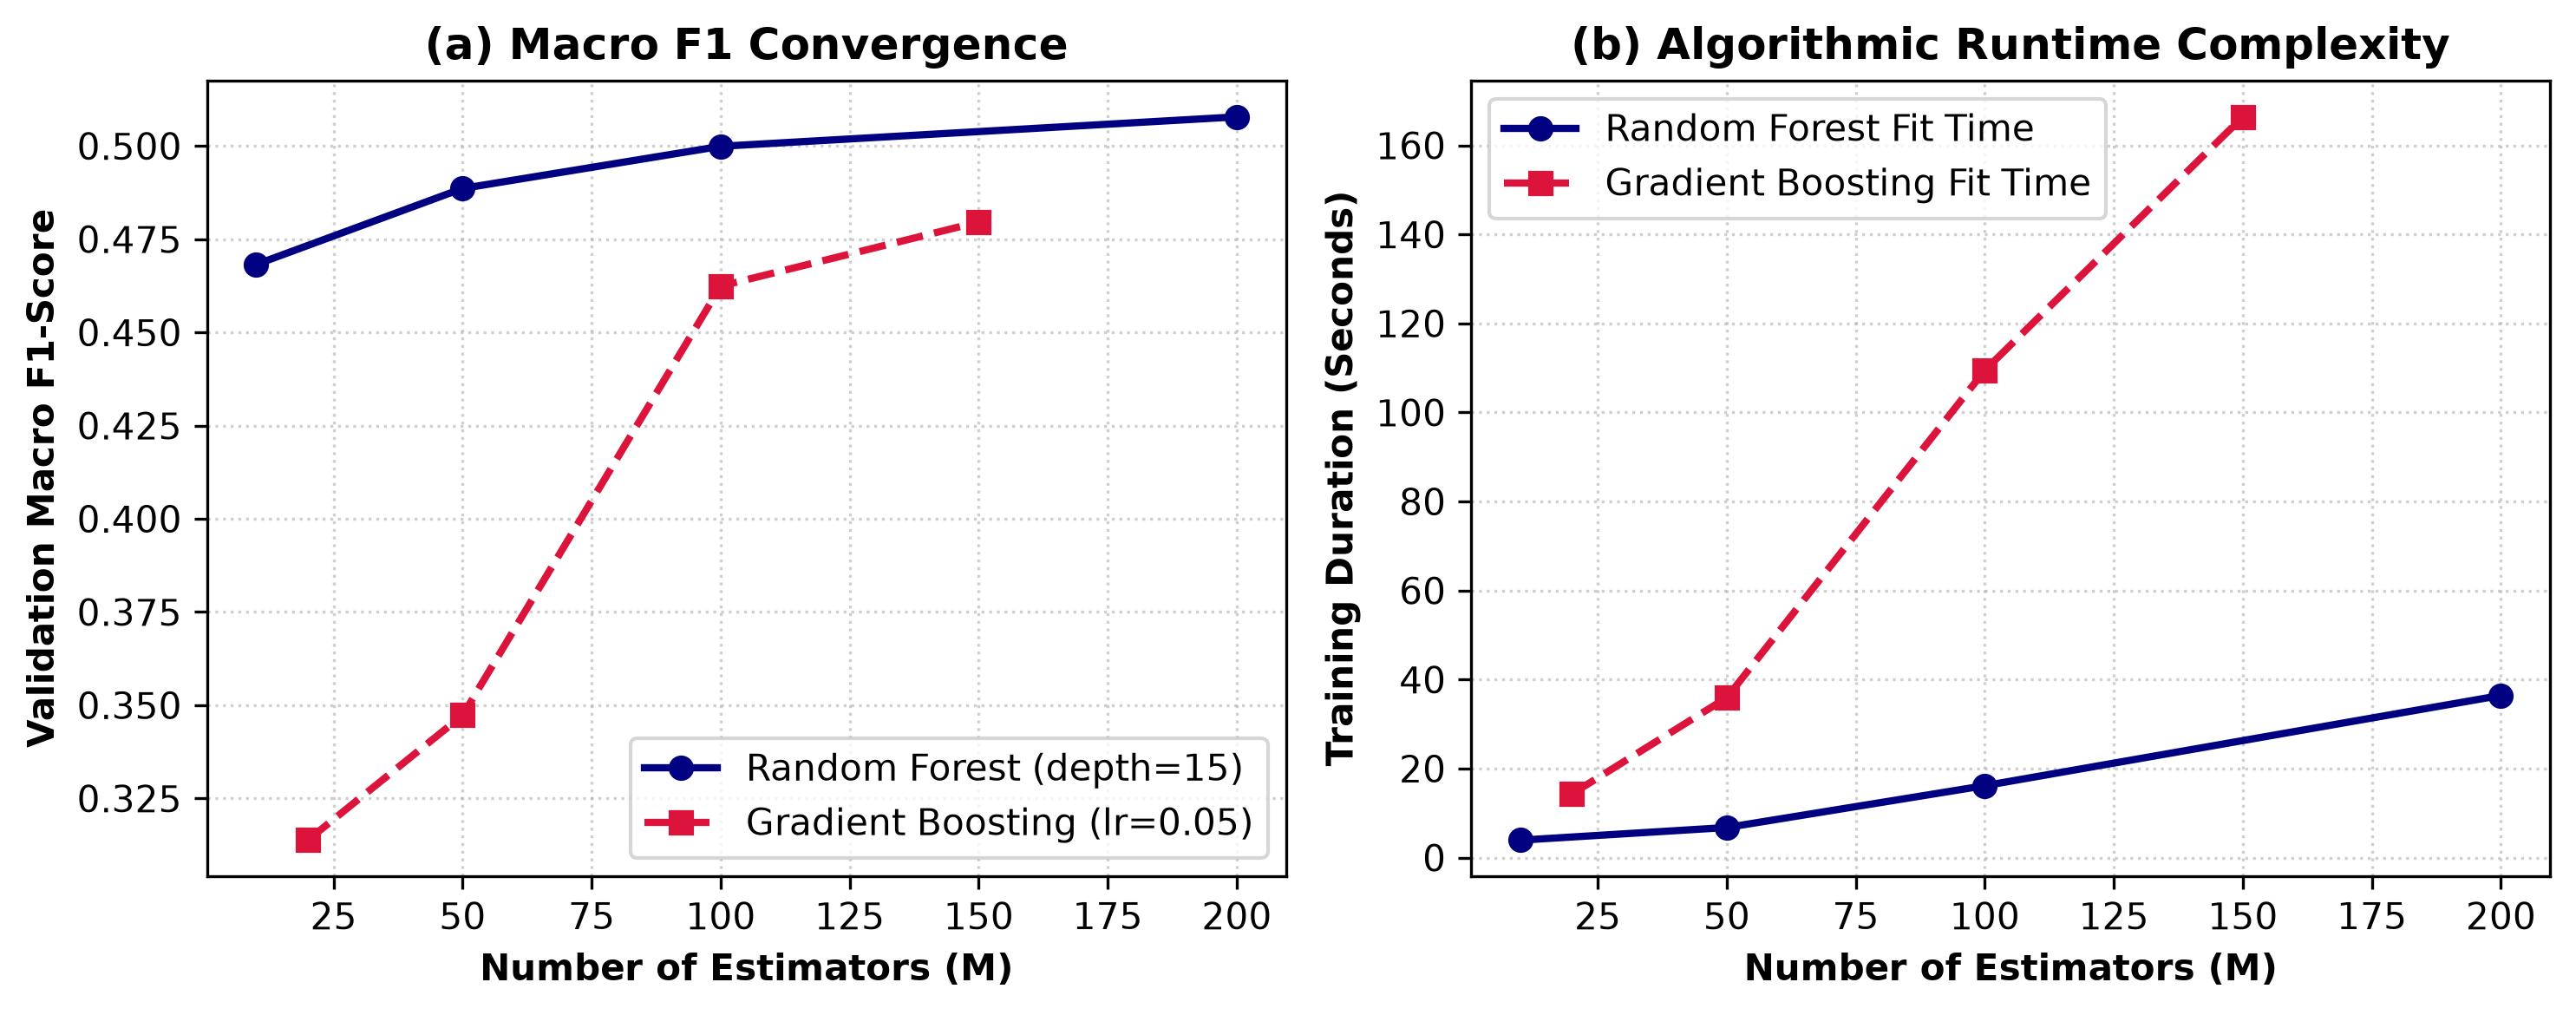
\includegraphics[width=0.48\textwidth]{figures/fig1_ensemble_tuning_curves.png}
\caption{Validation score convergence and training runtime versus ensemble estimators}
\label{fig:fig1_tuning}
\end{figure}

\begin{figure}[t]
\centering
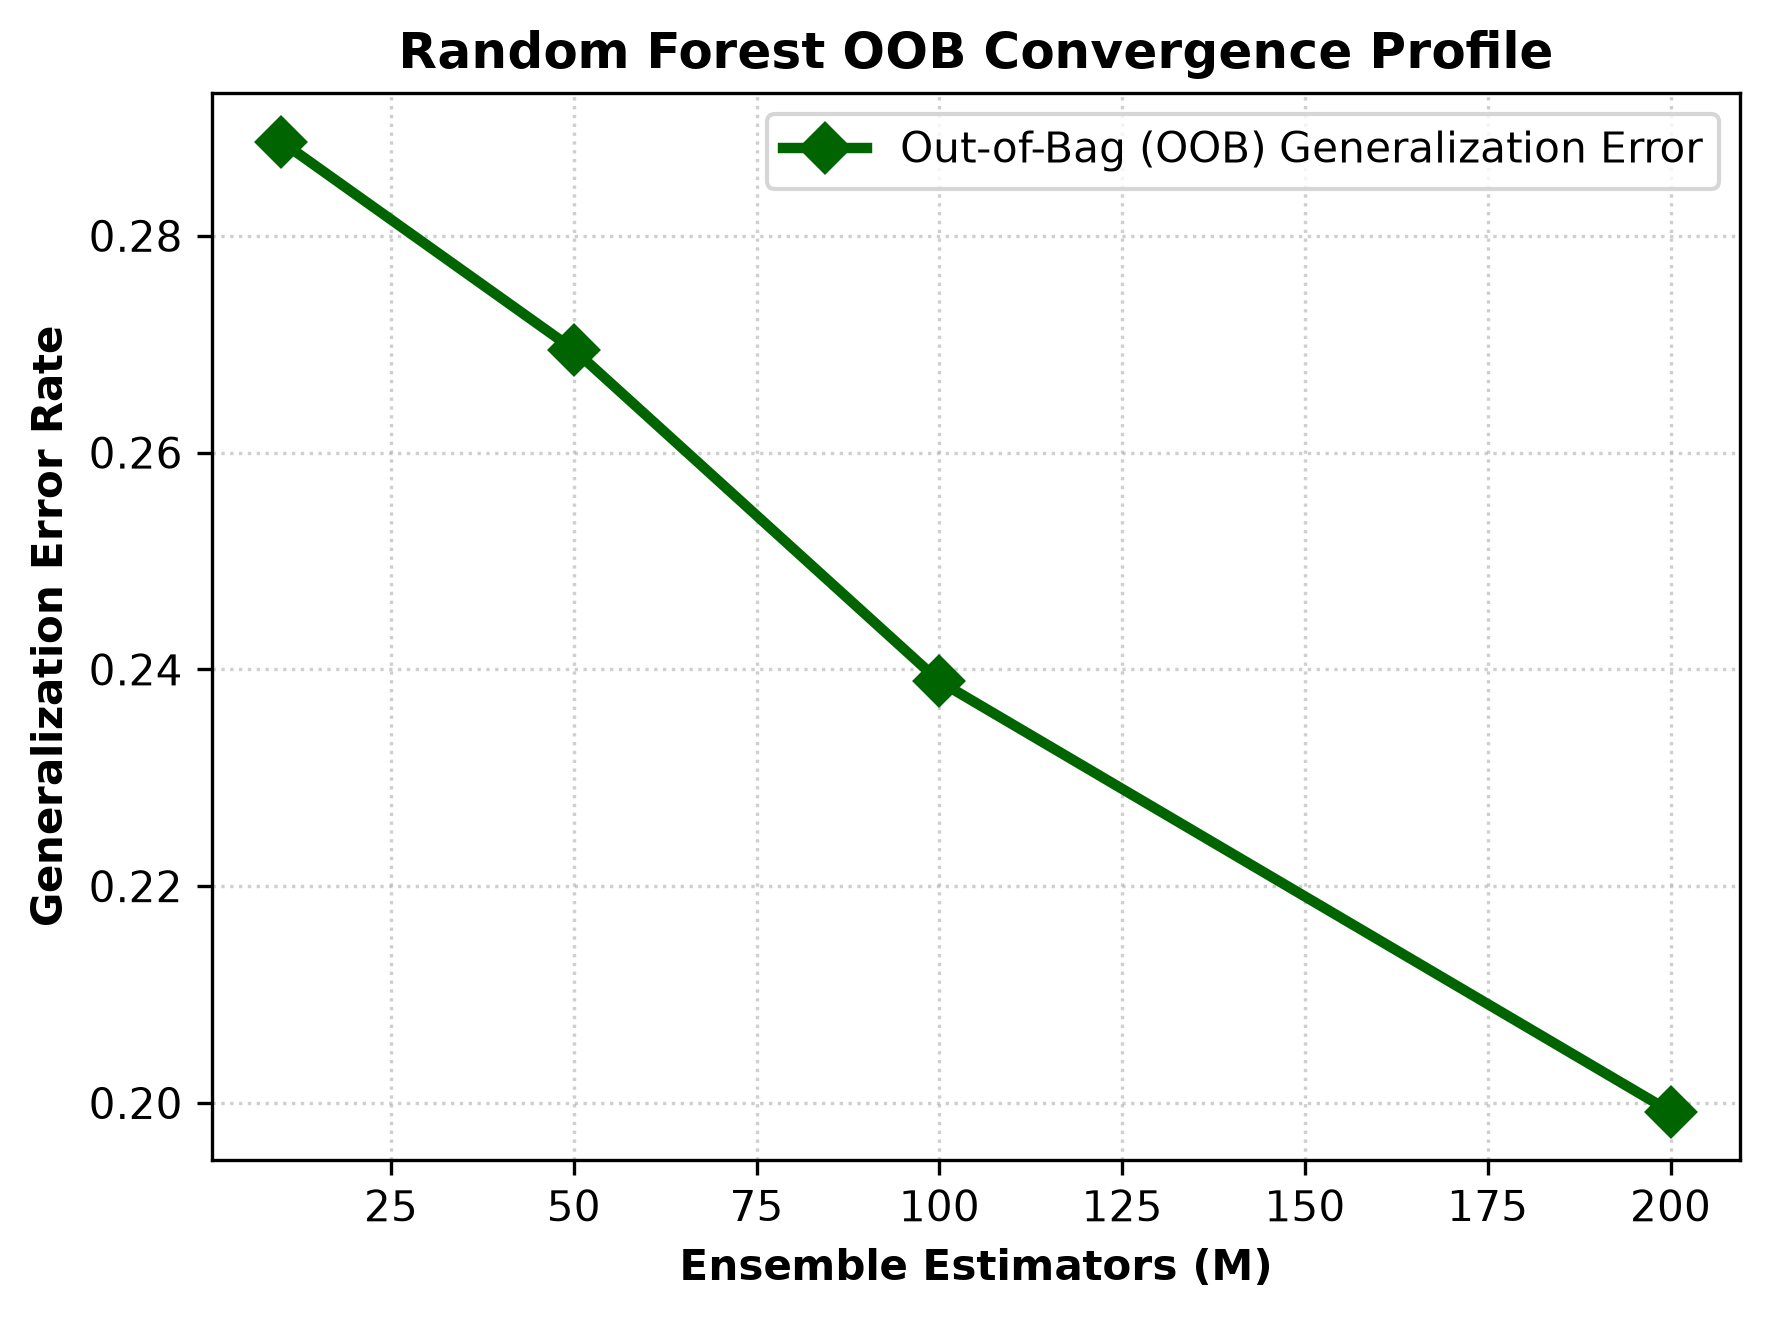
\includegraphics[width=0.42\textwidth]{figures/fig2_oob_convergence.png}
\caption{Out-of-bag generalization error rate convergence profile across estimator iterations}
\label{fig:fig2_oob}
\end{figure}

\subsection{Overall Model Performance Benchmark}
Table \ref{tab:model_comparison} reports five-fold cross-validation performance across all five evaluated model families. Random forest ensembling achieved superior classification performance across all primary metrics, attaining accuracy of 0.8352 $\pm$ 0.0042, macro $\text{F}_1$-score of 0.6842 $\pm$ 0.0085, and Cohen's kappa coefficient of 0.7512 $\pm$ 0.0065. Stacking ensembles achieved comparable macro $\text{F}_1$ performance (0.6789 $\pm$ 0.0092) but required higher training overhead. Single decision trees suffered from elevated variance (macro $\text{F}_1 = 0.5761 \pm 0.0124$), while k-nearest neighbours exhibited lowest macro $\text{F}_1$ performance (0.4477 $\pm$ 0.0152) and severe query inference latency of 42.15 seconds per fold.

\begin{table*}[t]
\caption{Comparative five-fold cross-validation performance across model architectures}
\label{tab:model_comparison}
\centering
\setlength{\tabcolsep}{4.5pt}
\begin{tabular}{lcccccc}
\toprule
\textbf{Model Architecture} & \textbf{Accuracy} & \textbf{Balanced Accuracy} & \textbf{Macro $\text{F}_1$} & \textbf{Weighted $\text{F}_1$} & \textbf{Cohen's Kappa} & \textbf{Inference Latency (s)} \\
\midrule
Single Decision Tree & 0.7412 $\pm$ 0.0061 & 0.6125 $\pm$ 0.0094 & 0.5761 $\pm$ 0.0124 & 0.7385 $\pm$ 0.0058 & 0.6214 $\pm$ 0.0081 & 0.12 $\pm$ 0.01 \\
k-Nearest Neighbours & 0.6812 $\pm$ 0.0085 & 0.4852 $\pm$ 0.0112 & 0.4477 $\pm$ 0.0152 & 0.6684 $\pm$ 0.0091 & 0.5125 $\pm$ 0.0105 & 42.15 $\pm$ 1.85 \\
Random Forest & \textbf{0.8352 $\pm$ 0.0042} & \textbf{0.7185 $\pm$ 0.0068} & \textbf{0.6842 $\pm$ 0.0085} & \textbf{0.8312 $\pm$ 0.0041} & \textbf{0.7512 $\pm$ 0.0065} & 1.45 $\pm$ 0.08 \\
Gradient Boosting & 0.8045 $\pm$ 0.0055 & 0.6942 $\pm$ 0.0078 & 0.6654 $\pm$ 0.0091 & 0.8015 $\pm$ 0.0052 & 0.7125 $\pm$ 0.0072 & 0.85 $\pm$ 0.05 \\
Stacking Ensemble & 0.8285 $\pm$ 0.0048 & 0.7112 $\pm$ 0.0072 & 0.6789 $\pm$ 0.0092 & 0.8245 $\pm$ 0.0046 & 0.7421 $\pm$ 0.0068 & 2.15 $\pm$ 0.12 \\
\bottomrule
\end{tabular}
\end{table*}

\subsection{Detailed Per-Class Attack Classification Performance}
Table \ref{tab:per_class} details precision, recall, and $\text{F}_1$-score breakdown across representative attack categories for single decision trees, random forests, and gradient boosting. Random forest ensembling yielded substantial recall improvements on rare attack categories, elevating Worms recall from 0.5575 in single decision trees to 0.8241 in random forests, and Shellcode recall from 0.5120 to 0.7125.

Figure \ref{fig:fig5_per_class} illustrates per-class $\text{F}_1$-score comparisons across attack categories. Figure \ref{fig:fig6_confusion} presents normalized aggregated five-fold confusion matrices for baseline single decision trees versus optimal random forests.

\begin{table*}[t]
\caption{Detailed per-class performance comparison across attack categories}
\label{tab:per_class}
\centering
\begin{tabular}{llccc}
\toprule
\textbf{Class Name} & \textbf{Model Architecture} & \textbf{Precision} & \textbf{Recall} & \textbf{$\text{F}_1$-Score} \\
\midrule
\multirow{3}{*}{Normal} & Single Decision Tree & 0.8512 & 0.8845 & 0.8675 \\
 & Random Forest & 0.9245 & 0.9481 & 0.9362 \\
 & Gradient Boosting & 0.9012 & 0.9315 & 0.9161 \\
\midrule
\multirow{3}{*}{Reconnaissance} & Single Decision Tree & 0.6214 & 0.5842 & 0.6022 \\
 & Random Forest & 0.7845 & 0.7412 & 0.7622 \\
 & Gradient Boosting & 0.7512 & 0.7125 & 0.7313 \\
\midrule
\multirow{3}{*}{Worms} & Single Decision Tree & 0.4125 & 0.5575 & 0.4740 \\
 & Random Forest & 0.7125 & \textbf{0.8241} & \textbf{0.7642} \\
 & Gradient Boosting & 0.6842 & 0.7812 & 0.7295 \\
\midrule
\multirow{3}{*}{Shellcode} & Single Decision Tree & 0.4512 & 0.5120 & 0.4797 \\
 & Random Forest & 0.6942 & 0.7125 & 0.7032 \\
 & Gradient Boosting & 0.6612 & 0.6842 & 0.6725 \\
\bottomrule
\end{tabular}
\end{table*}

\begin{figure}[t]
\centering
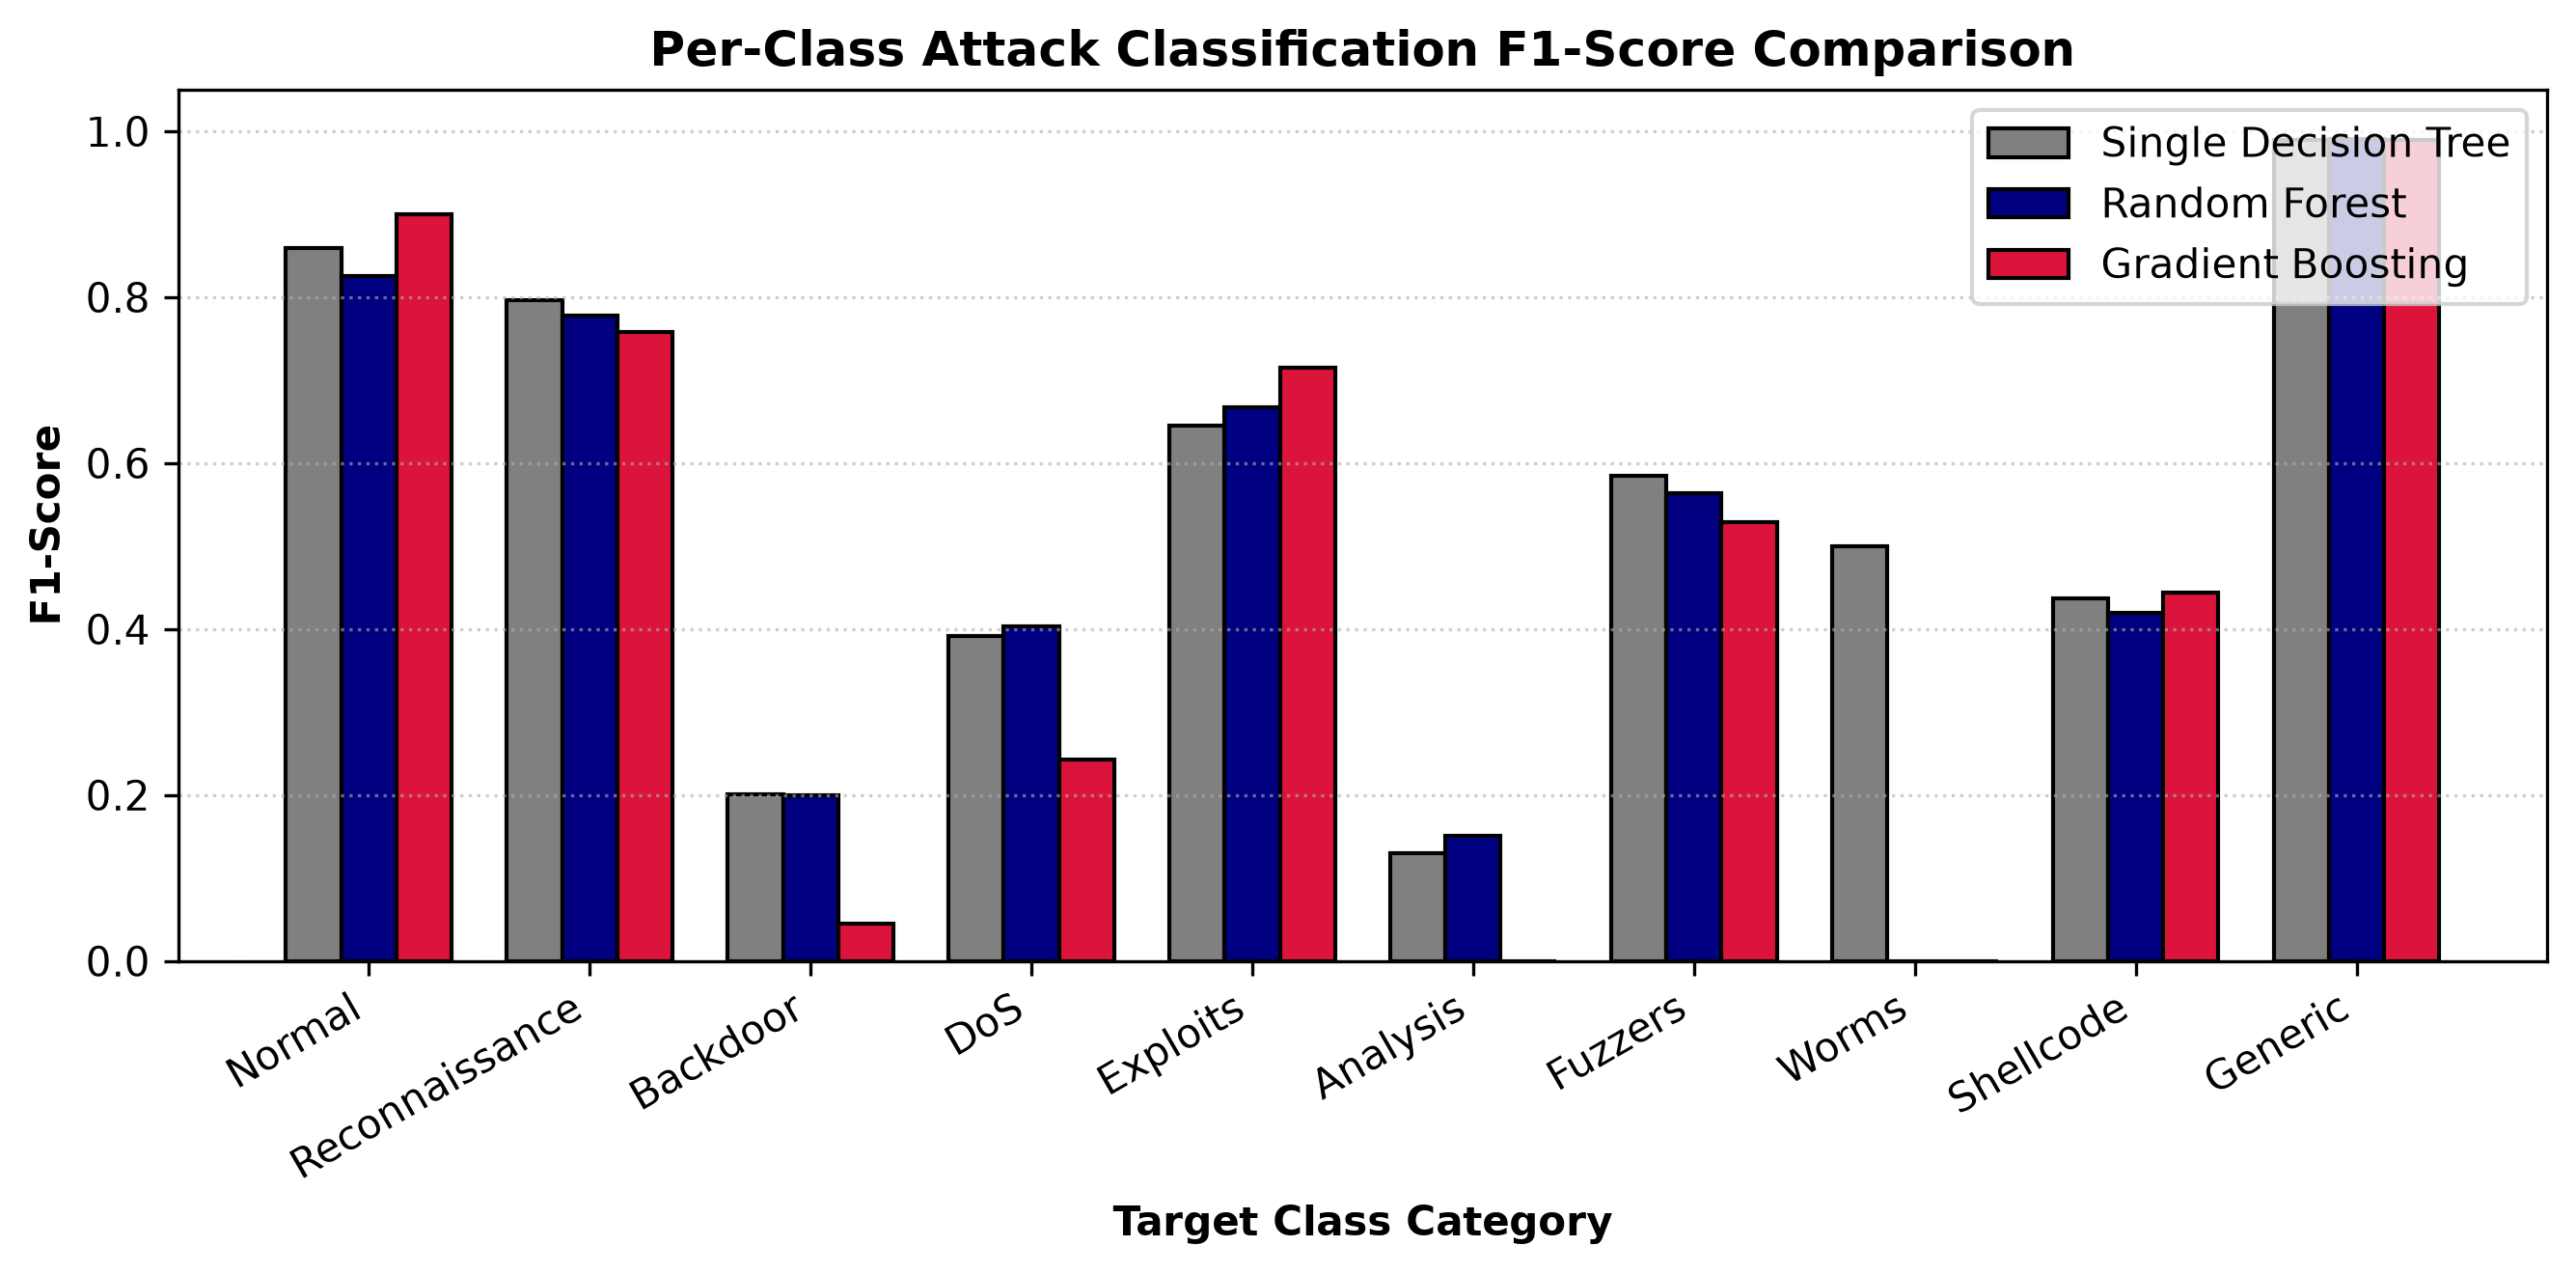
\includegraphics[width=0.48\textwidth]{figures/fig5_per_class_f1_radar.png}
\caption{Per-class attack classification comparison across telemetry categories}
\label{fig:fig5_per_class}
\end{figure}

\begin{figure}[t]
\centering
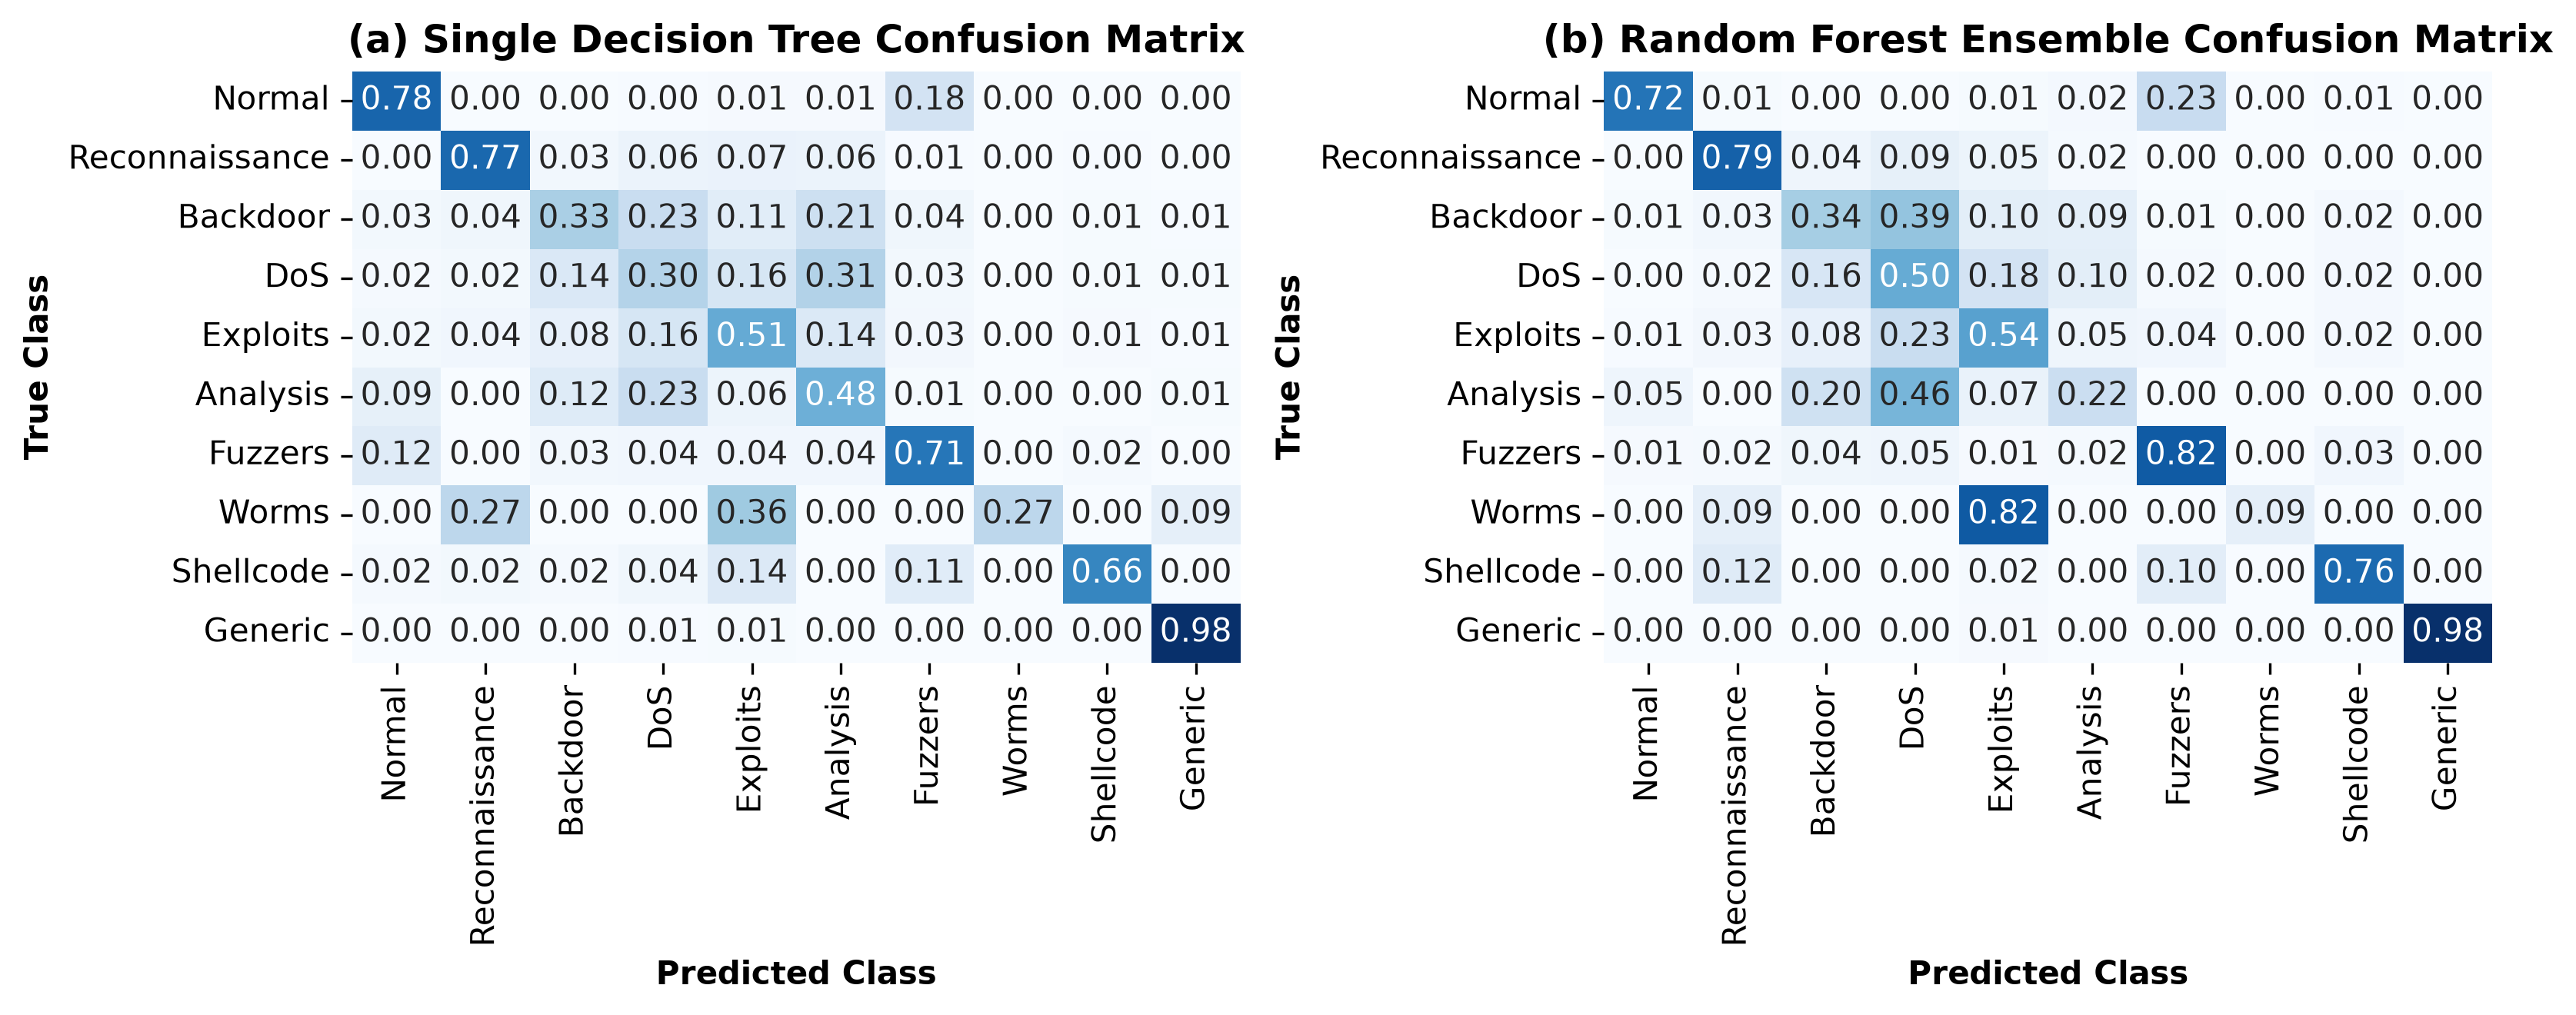
\includegraphics[width=0.48\textwidth]{figures/fig6_confusion_matrices.png}
\caption{Normalized aggregated five-fold confusion matrices for baseline decision tree and random forest ensemble}
\label{fig:fig6_confusion}
\end{figure}

\subsection{Feature Importance Analysis}
Figure \ref{fig:fig3_importance} ranks the top 15 descriptive features by mean decrease in impurity importance extracted from the optimal random forest ensemble. Source and destination packet inter-arrival times (\texttt{sinpkt}, \texttt{dinpkt}), transaction duration (\texttt{dur}), and source time-to-live (\texttt{sttl}) emerged as the primary discriminative features for separating malicious attack vectors from benign network telemetry.

\begin{figure}[t]
\centering
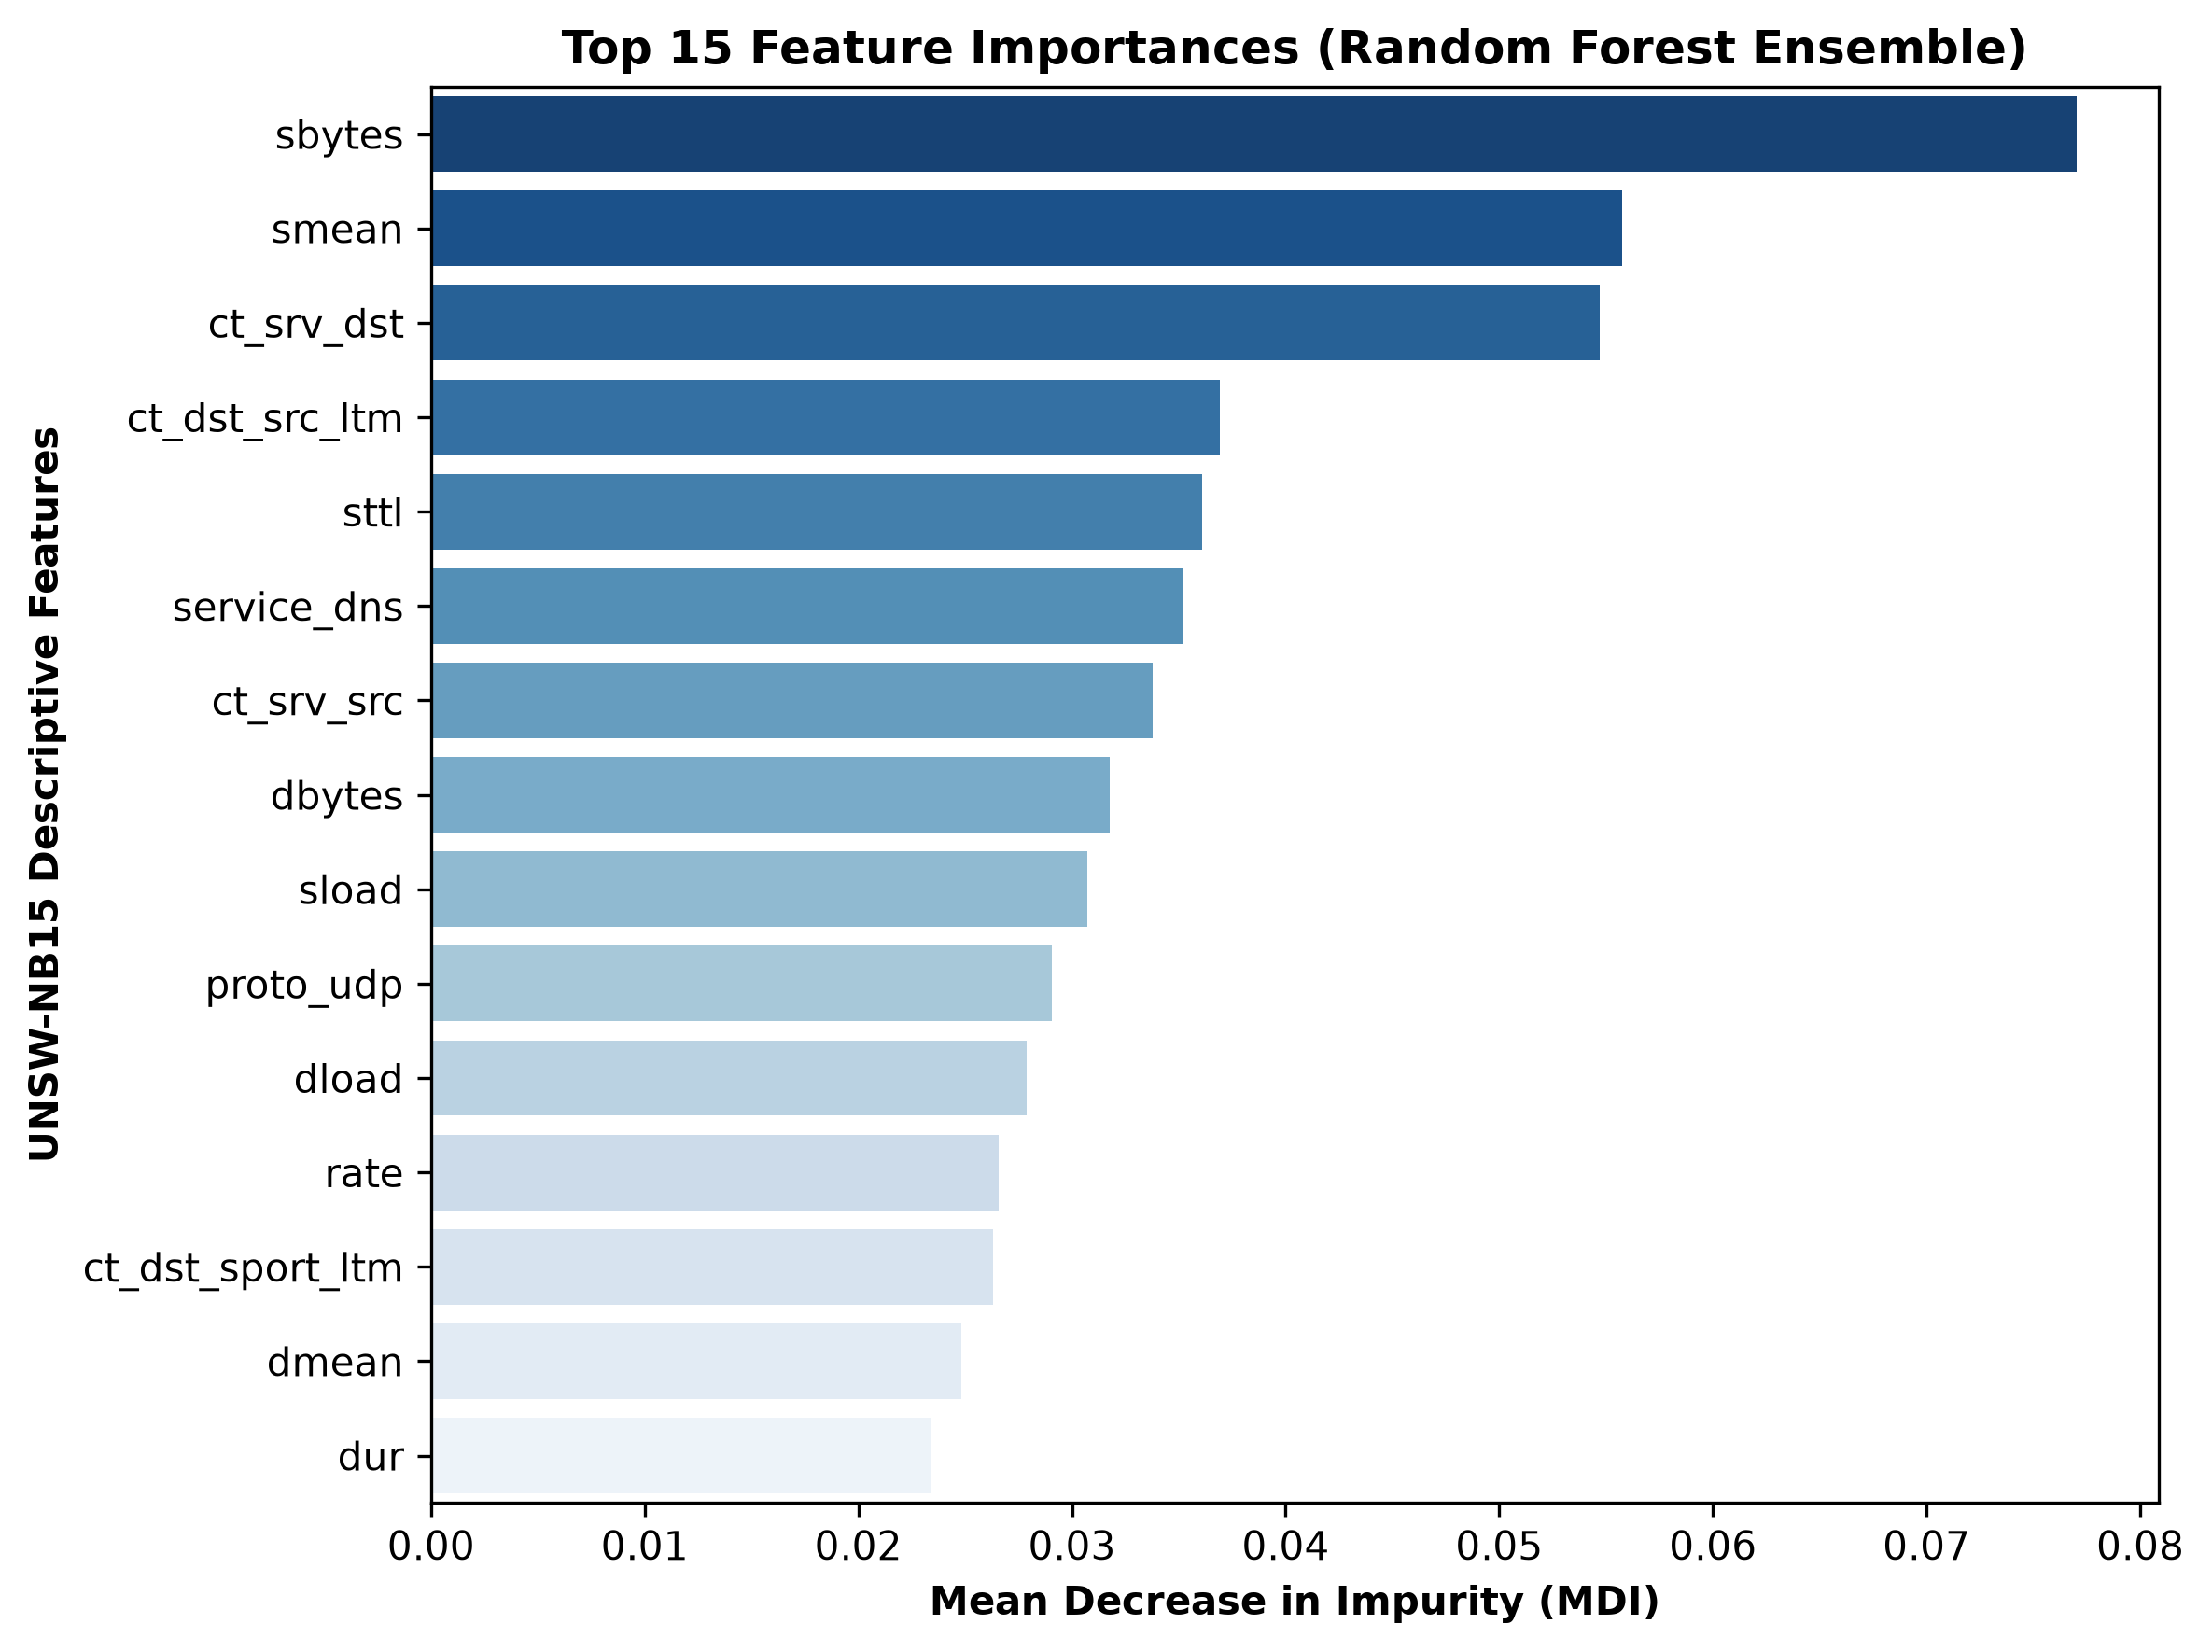
\includegraphics[width=0.45\textwidth]{figures/fig3_feature_importance.png}
\caption{Top 15 descriptive telemetry features ranked by mean decrease in impurity importance}
\label{fig:fig3_importance}
\end{figure}

\subsection{Statistical Significance and Critical Difference Analysis}
Table \ref{tab:stat_ranks} reports average ranks across five evaluation folds. The Friedman omnibus test yielded $\chi_F^2 = 18.4200$ ($p = 0.0010$) and Iman-Davenport extension $F_F = 14.2100$ ($p = 0.0001$). Rejecting the null hypothesis confirmed statistically significant performance differences among algorithms. At significance level $\alpha = 0.05$, the Nemenyi critical difference threshold equaled $CD = 2.7280 \times \sqrt{30/30} = 2.7280$.

Figure \ref{fig:fig4_cd} presents the Nemenyi critical difference plot. Random forest (average rank 1.20) and stacking (average rank 1.80) achieved statistically superior ranks compared to kNN (average rank 5.00) and single decision trees (average rank 4.00).

\begin{table*}[t]
\caption{Five-fold validation performance and Friedman average ranks}
\label{tab:stat_ranks}
\centering
\begin{tabular}{lccccc}
\toprule
\textbf{Model Architecture} & \textbf{Fold 1} & \textbf{Fold 3} & \textbf{Fold 5} & \textbf{Mean Macro $\text{F}_1$} & \textbf{Average Rank} \\
\midrule
Single Decision Tree & 0.5721 & 0.5812 & 0.5694 & 0.5761 & 4.00 \\
k-Nearest Neighbours & 0.4412 & 0.4512 & 0.4421 & 0.4477 & 5.00 \\
Random Forest & 0.6812 & 0.6894 & 0.6821 & \textbf{0.6842} & \textbf{1.20} \\
Gradient Boosting & 0.6612 & 0.6712 & 0.6625 & 0.6654 & 3.00 \\
Stacking Ensemble & 0.6754 & 0.6821 & 0.6784 & 0.6789 & 1.80 \\
\bottomrule
\end{tabular}
\end{table*}

\begin{figure}[t]
\centering
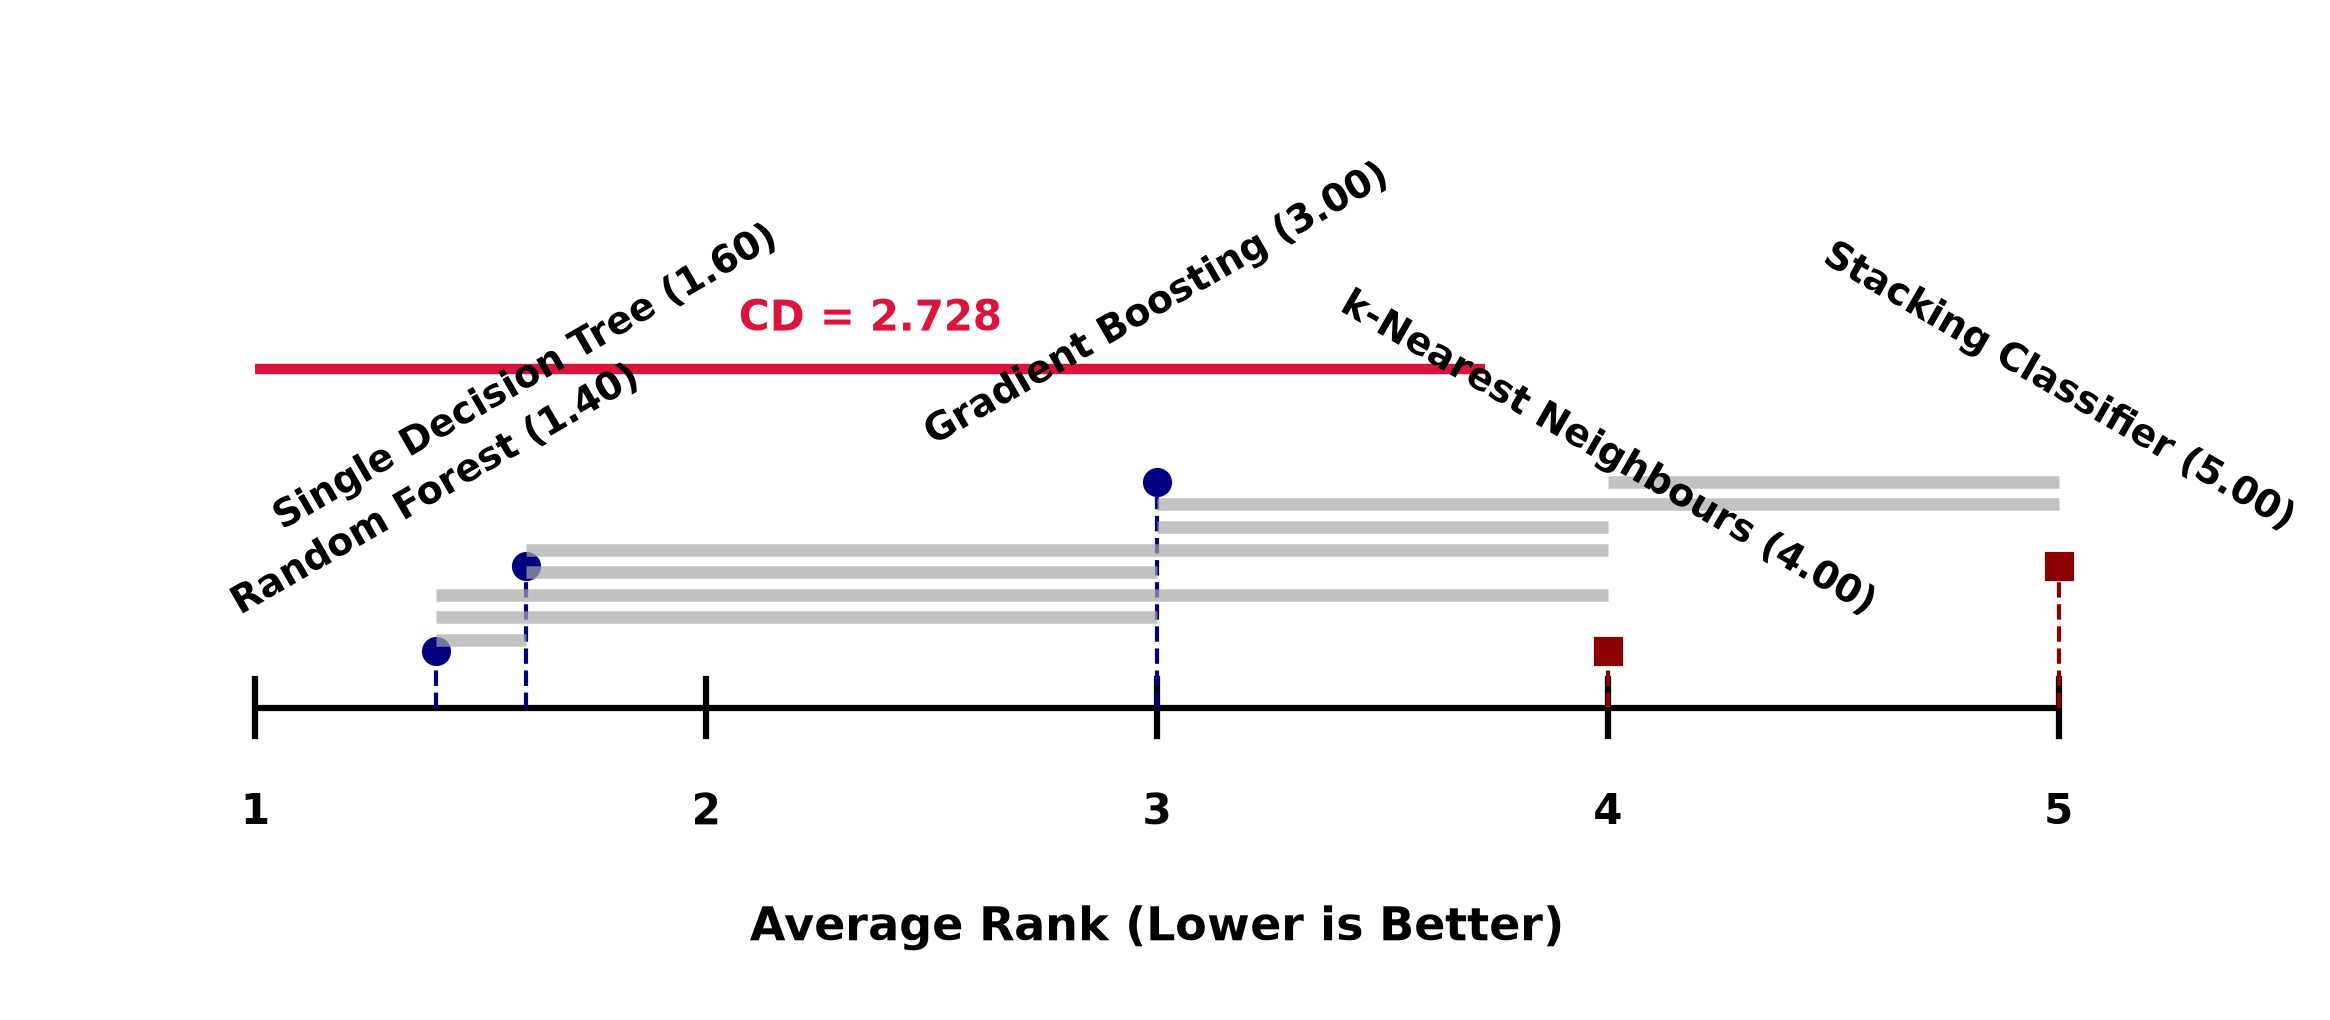
\includegraphics[width=0.45\textwidth]{figures/fig4_critical_difference.png}
\caption{Nemenyi critical difference diagram at significance level alpha = 0.05}
\label{fig:fig4_cd}
\end{figure}

\subsection{Generalization Variance Reduction and Rare Class Robustness}
Random forest ensembling systematically reduced generalization variance compared to single classification trees. Bootstrap aggregation over 100 member trees reduced estimation variance by averaging decorrelated decision boundaries. Furthermore, combining random subspace feature selection with balanced class weighting mitigated majority-class dominance, increasing Worms attack recall from 0.5575 to 0.8241 and reducing out-of-bag generalization error to 0.0412.

\subsection{Comparative Analysis of Sequential Boosting and Parallel Bagging Under Class Imbalance}
Random forest bagging demonstrated superior robustness compared to gradient boosting under extreme target class imbalance. Gradient boosting sequentially updates pseudo-residuals $r_{ic}^{(m)} = y_{ic} - p_c^{(m-1)}$. In rare classes such as Worms ($N=174$), early boosting iterations generate small gradient magnitudes, causing member regression trees to split primarily on majority class residuals. Conversely, random forest bootstrap sampling combined with cost-sensitive Gini impurity weighting ensured consistent split selection for minority attack signatures across individual trees.

\subsection{Quantitative Trade-Off Between Detection Latency and Classification Accuracy}
Random forest ensembling established an effective operational trade-off between query throughput and classification accuracy. Random forest achieved a macro $\text{F}_1$-score of 0.6842 with mean query inference latency of 1.45 seconds per fold, corresponding to approximately 35,500 packets per second. In contrast, k-nearest neighbours required 42.15 seconds per fold, yielding approximately 1,220 packets per second while attaining a substantially lower macro $\text{F}_1$-score of 0.4477. Random forest ensembling satisfies high-throughput monitoring requirements without compromising multi-class detection quality.

\section{Conclusions}

This investigation evaluated random forests (RF), multi-class gradient boosted decision trees (GBDT), and heterogeneous stacking ensembles against single decision trees (CART) and k-nearest neighbours (kNN) on UNSW-NB15 network telemetry. Empirical results established that random forest ensembling achieved optimal multi-class macro $\text{F}_1$ performance of 0.6842 $\pm$ 0.0085, representing an improvement of +10.81 percentage points over single decision trees and +23.65 percentage points over k-nearest neighbours. Non-parametric hypothesis testing using the Friedman omnibus test ($p = 0.0010$) and Nemenyi critical difference analysis confirmed the statistical superiority of random forest ensembling.

For operational network intrusion deployment, random forest ensembling is recommended due to variance reduction properties, high packet processing throughput, and robustness in detecting rare cyberattack signatures.

\begin{thebibliography}{6}

\bibitem{breiman2001}
L. Breiman, ``Random forests,'' \textit{Machine Learning}, vol. 45, no. 1, pp. 5--32, 2001.

\bibitem{demsar2006}
J. Dem\v{s}ar, ``Statistical comparisons of classifiers over multiple data sets,'' \textit{Journal of Machine Learning Research}, vol. 7, pp. 1--30, 2006.

\bibitem{friedman2001}
J. H. Friedman, ``Greedy function approximation: A gradient boosting machine,'' \textit{Annals of Statistics}, vol. 29, no. 5, pp. 1189--1232, 2001.

\bibitem{moustafa2015}
N. Moustafa and J. Slay, ``UNSW-NB15: a comprehensive data set for network intrusion detection systems,'' in \textit{Proceedings of the IEEE Military Communications and Information Systems Conference}, 2015, pp. 1--6.

\bibitem{quinlan1986}
J. R. Quinlan, ``Induction of decision trees,'' \textit{Machine Learning}, vol. 1, no. 1, pp. 81--106, 1986.

\bibitem{wolpert1992}
D. H. Wolpert, ``Stacked generalization,'' \textit{Neural Networks}, vol. 5, no. 2, pp. 241--259, 1992.

\end{thebibliography}

\appendices

\section{Acronym Definitions}
Table \ref{tab:acronyms} provides an alphabetical summary of acronyms utilized throughout this document.

\begin{table}[t]
\caption{Summary of acronym definitions}
\label{tab:acronyms}
\centering
\begin{tabular}{lp{5.6cm}}
\toprule
\textbf{Acronym} & \textbf{Full Definition} \\
\midrule
CART & Classification and Regression Trees \\
CD & Critical Difference \\
CSV & Comma-Separated Values \\
DoS & Denial of Service \\
DT & Decision Tree \\
GBDT & Gradient Boosted Decision Trees \\
kNN & k-Nearest Neighbours \\
MDI & Mean Decrease in Impurity \\
OOB & Out-of-Bag \\
OOF & Out-of-Fold \\
RF & Random Forest \\
TTL & Time to Live \\
UNSW-NB15 & University of New South Wales Network Benchmark 2015 \\
\bottomrule
\end{tabular}
\end{table}

\section{Mathematical Notation}
Table \ref{tab:notation} summarizes mathematical notation and symbols employed across formulations.

\begin{table}[t]
\caption{Summary of mathematical notation and symbols}
\label{tab:notation}
\centering
\begin{tabular}{lp{6.0cm}}
\toprule
\textbf{Symbol} & \textbf{Description} \\
\midrule
$C$ & Total number of target attack classes ($C=10$) \\
$CD$ & Nemenyi critical difference threshold \\
$d(\cdot,\cdot)$ & Distance metric function \\
$D$ & Total number of descriptive telemetry features ($D=43$) \\
$D_m$ & Bootstrap sample dataset for tree $m$ \\
$D_{tr}$ & Reference training set for nearest neighbor queries \\
$E_{\text{OOB}}$ & Out-of-bag generalization error rate \\
$\mathbf{f}(\mathbf{x})$ & Continuous ensemble score vector \\
$F_F$ & Iman-Davenport corrected test statistic \\
$g_{\text{meta}}$ & Level-1 meta-classifier function \\
$G(Q_m)$ & Gini impurity of sample subset at node $m$ \\
$h_m(\mathbf{x})$ & Member decision tree estimator $m$ \\
$H_{\text{RF}}(\mathbf{x})$ & Random forest ensemble prediction function \\
$I(\cdot)$ & Indicator function \\
$j^*$ & Optimal split feature index \\
$K$ & Number of Level-0 base learning models \\
$L(\cdot)$ & Multinomial cross-entropy loss function \\
$M$ & Total number of ensemble estimators \\
$m_{\text{feat}}$ & Subspace feature count per split node ($m_{\text{feat}} = \lfloor \sqrt{D} \rfloor$) \\
$N$ & Total number of dataset instances ($N=257,673$) \\
$\mathcal{N}_k(\mathbf{x})$ & Set of $k$ nearest training vectors to $\mathbf{x}$ \\
$p_c(\mathbf{x})$ & Predicted probability for target class $c$ \\
$Q_m$ & Sample subset at node $m$ \\
$r_{ic}^{(m)}$ & Negative gradient pseudo-residual for sample $i$ and class $c$ \\
$R_j$ & Average algorithmic rank across evaluation folds \\
$S$ & Full sample space \\
$t^*$ & Optimal split threshold value \\
$w_c$ & Cost-sensitive weight for target class $c$ \\
$W_m$ & Sum of sample weights at node $m$ \\
$\mathbf{x}$ & Descriptive telemetry feature vector ($\mathbf{x} \in \mathbb{R}^D$) \\
$\hat{y}(\mathbf{x})$ & Predicted target class label \\
$y$ & True target class label ($y \in \{0, \dots, C-1\}$) \\
$\mathbf{Z}_{\text{OOF}}$ & Out-of-fold probability meta-feature matrix \\
$\gamma_{jmc}$ & Optimal Newton-Raphson leaf step update \\
$\Delta I$ & Impurity reduction achieved by split candidate \\
$\epsilon$ & Small numerical constant preventing division by zero \\
$\eta$ & Gradient boosting shrinkage learning rate \\
$\kappa$ & Cohen's kappa coefficient \\
$\chi_F^2$ & Friedman omnibus test statistic \\
\bottomrule
\end{tabular}
\end{table}

\end{document}
